\section{Latency Assessments when Using Multiple Acquisition Sources}

\subsection*{Motivation and Objective}

Technological advancements in the field of sensory devices have allowed the collection of various bodily signals such as Acceleration (ACC), Electrocardiogram (ECG), Electromyogram (EMG), and Electrodermal Activity (EDA) using discrete wearable devices. These data streams can be used to validate semantic emotional descriptors based on valence and arousal measurements, linked to the user’s involuntary reactions transmitted by the Autonomic Nervous System (ANS). Where researchers may need to acquire data from many sources at once, we evaluate the use of the BITalino R-IoT, a low-cost sensory device designed for monitoring physiological activity in real-time.

A crucial feature we want researchers to be able to exploit is the ability to acquire and process data from multiple devices simultaneously. This can be configured to monitor the activity of many users or even to place sensors on additional body parts (to track movement from different limbs, for example). To benchmark the hardware capabilities of the device in experimental environments, we carry out tests to evaluate performance, outlining the absolute and relative latency in different conditions. These tests consider the effect of including additional devices to the network and differences in wireless range of data transmission.

\subsection{Preliminary Results}

In our tests, we calculate the time taken for the host computer to receive a response to a stimulus which changes in the analog input on the R-IoT device, which continuously sends data back to the host computer over a shared Wi-Fi network using the Open Sound Control (OSC) protocol. The stimulus signal is distributed to multiple devices which are included in the network to see the effect this has on latency. In addition, tests are performed to evaluate the impact of increasing the wireless communication distance from 1 metre to 5 metres. The test is run for a duration of several minutes to assess how the latency deviates over time.
Results show that as a base-latency, using one device at a placed a metre away from the wireless receiver, we calculated a mean latency of 8.9 milliseconds (ms). This increased to 10.7ms as the distance increased to 5 metres. When we included 4 devices, we saw a 1.1ms average increase in latency at 1 metre and 1.3ms at 5 metres. The average difference in latency among the devices was calculated as 3.2ms and 5.9ms respectively. The latency measurements were deemed stable over the time period of the test with no observable trend.

We found a slight increase in latency when using more devices on one network and as we increased the distance. Whilst this should be taken account for data synchronisation tasks, we would consider the BITalino R-IoT to be a suitable device for studies collecting physiological data from multiple sources. Our tests also support the use of the OSC protocol for this purpose.

\subsection{An Overview of the BITalino R-IoT}
\label{subsec:riot}

\subsection*{Device Overview}

The BITalino R-IoT module is the 7th generation of IRCAM's wireless sensor digitizing unit \cite{noauthor_bitalino_nodate}, an essential tool linking motion sensing, gestural recognition and Live Performance Arts. Since 2001, IRCAM aimed to provide a low latency, high data-rate \& resolution and stage compatible devices, capable of streaming gestural information to the computer from multiple performers. The BITalino R-IoT embeds a 9-axis digital IMU sensor (LSM9DS1) featuring a 3-axis accelerometer, a 3-axis gyroscope and a 3-axis magnetometer, allowing for instance the onboard computation of the absolute orientation of the module in space \cite{matzka_developing_2019}. The sensor is attached to the SPI port to sample the 16-bit motion data at high speed. In addition to this, there are two 12-bit ADC inputs, compatible with the BITalino sensor modules. Throughout this chapter, we refer to the BITalino R-IoT as R-IoT.

\subsection*{Wireless Communication Methods}

Out of the box, the R-IoT is programmed to transmit data over Wi-Fi through the Open Sound Control (OSC)\footnote{Open Sound Control: \url{http://opensoundcontrol.org/}} protocol. With the default configuration, each device will send an array of 21 float values every 5 milliseconds. This array includes motion data from the 9-axis IMU, as well as the analog inputs when are coupled with an OSC message address that includes the ID number of the device. We can assign individual ID numbers to each device in the network to separate the incoming data within the host computer.
% This is a protocol for communication among computers, sound synthesizers, and other multimedia devices that is optimised for modern networking technology (OSC).
% The main features include the following:
% \begin{itemize}
%   \item Open-ended, dynamic, URL-style symbolic naming scheme
%   \item Symbolic and high-resolution numeric argument data
%   \item Pattern matching language to specify multiple recipients of a single message
%   \item High resolution time tags
%   \item 'Bundles' of messages whose effects must occur simultaneously
% \end{itemize}

\subsection{Experimental Protocol}

In our tests, we calculate the time taken for the host computer to receive a response to a stimulus which changes in the analog input on the R-IoT device. The stimulus signal is distributed to multiple devices which are included in the network to see the effect this has on latency. The test is run for a duration of several minutes to assess how the latency deviates over time.

\subsection*{Reference Signal and Timestamps}
The stimulus signal is originally triggered from the host computer, which sends single byte messages to a Teensy 3.2 board\footnote{Teensy 3.2: \url{https://www.pjrc.com/store/teensy32.html}} via USB serial. Upon receiving a message from the host computer, the Teensy board will output either 3.3 or 0 volts that is put through a voltage divider before reaching the analog input of the R-IoT device. The R-IoT then sends OSC packets (containing the analog input value) back to the host computer via a TP-Link MR3020 Wi-Fi router. The stimulus is set to switch every second, resulting in an oscillation of 0.5 Hz (Figure \ref{fig:latency_fig1}).

% Figure 1
\begin{figure}[htbp]
  \centering
    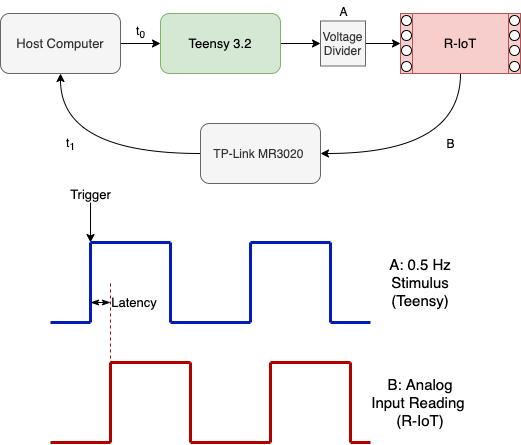
\includegraphics[width=0.7\textwidth]{Chapters/Figures/technical/Latency/figure1.png}
    \caption{Experimental protocol for latency tests.}
    \label{fig:latency_fig1}
\end{figure}

A timestamp is logged at t\textsubscript{0}, the moment the trigger message is sent from the host computer. Another is logged at t\textsubscript{1}, when the change is received in the incoming OSC message. From here, we define the latency as t\textsubscript{1} – t\textsubscript{0} for each instance of a trigger message. This approach is partially inspired by the closed-loop latency tests performed by Sebastian Madgwick for the x-OSC device \cite{madgwick_x-osc_2013}, where a square wave is fed into the analog input of the device and outputted into a frequency counter to measure latency. We acknowledge that this method is not as accurate due to the small latency that occurs between the host computer and the Teensy, addressed in Section \ref{subsec:latency_limitations}. However, we consider this a low-cost solution that can be more easily replicated for the user’s specific conditions and environment.

% \subsubsubsection{Multiple Device Setup}
\subsection*{Multiple Device Setup}
To test multiple devices simultaneously, we feed the same reference signal from the Teensy to many R-IoTs, as shown in Figure \ref{fig:latency_fig2}. The devices are configured to stream data through the same Wi-Fi router, where the data is addressed by the ID number of each device.

\begin{figure}[htbp]
  \centering
    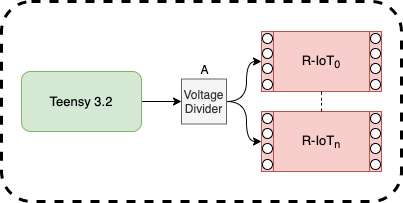
\includegraphics[width=0.7\textwidth]{Chapters/Figures/technical/Latency/figure2.png}
    \caption{Feeding reference signal to multiple R-IoTs.}
    \label{fig:latency_fig2}
\end{figure}

\subsection*{Device Firmware}
Each device is flashed with the default firmware, which implements algorithms to compute the absolute orientation of the device from the raw IMU data, providing quaternions and Euler angles every time a data packet is transmitted. For this reason, our tests can be considered to account for the latency that occurs when retrieving motion data.

\subsection{Results \& Discussion}

\subsection*{Conditions}
For these tests, the device(s) were first placed less than 1 metre away from the router which was connected to the host via an ethernet connection. From the test, we extracted 248 triggers form a total duration of approximately 8 minutes and 15 seconds. We then repeated the tests with the device(s) placed 5 metres away from the router.

\subsection*{Single Device}
% \subparagraph{Data Analysis}
For the duration of the test, we accumulate the latencies for every trigger and calculate a minimum, maximum and mean average latency. The results are given in Table \ref{table:latency_tab1}, ranging between 6 to 11 milliseconds. When we repeat the test at greater distance, we see a greater range of values and a higher average, as shown in Table \ref{table:latency_tab2} and Figure \ref{fig:latency_fig3}. Over the duration of the acquisitions, we could not observe any increasing/decreasing trend in the results.

% % Table 1
% \begin{table}[!h]
%     \centering
%     \begin{tabular}{*{4}{l}}\hline
%     % \rowcolor[HTML]{34CDF9}
%     \textbf{Device ID} & \textbf{\begin{tabular}[c]{@{}l@{}}Maximum\\ Latency (ms)\end{tabular}} & \textbf{\begin{tabular}[c]{@{}l@{}}Minimum\\ Latency (ms)\end{tabular}} & \textbf{\begin{tabular}[c]{@{}l@{}}Mean\\ Latency (ms)\end{tabular}} \\
%     \\[-1em]
%     \hline
%     \\[-1em]
%     0                  & 11.019                        & 6.605                & 8.859\\
%     \\[-1em]
%     \hline
%     \end{tabular}
% \caption{Latency results for one device (1 metre).}
% \label{table:latency_tab1}
% \end{table}

% % Table 2
% \begin{table}[!h]
%     \centering
%     \begin{tabular}{*{4}{l}}\hline
%     % \rowcolor[HTML]{34CDF9}
%     \textbf{Device ID} & \textbf{\begin{tabular}[c]{@{}l@{}}Maximum\\ Latency (ms)\end{tabular}} & \textbf{\begin{tabular}[c]{@{}l@{}}Minimum\\ Latency (ms)\end{tabular}} & \textbf{\begin{tabular}[c]{@{}l@{}}Mean\\ Latency (ms)\end{tabular}} \\
%     \\[-1em]
%     \hline
%     \\[-1em]
%     0                  & 11.019                        & 6.605                & 8.859\\
%     \\[-1em]
%     \hline
%     \end{tabular}
% \caption{Latency results for one device (1 metre).}
% \label{table:latency_tab2}
% \end{table}

\begin{table}[htbp]
    \begin{subtable}[c]{\textwidth}
        \centering
            \begin{tabular}{*{4}{l}}\hline
            % \rowcolor[HTML]{34CDF9}
            \textbf{Device ID} & \textbf{\begin{tabular}[c]{@{}l@{}}Maximum\\ Latency (ms)\end{tabular}} & \textbf{\begin{tabular}[c]{@{}l@{}}Minimum\\ Latency (ms)\end{tabular}} & \textbf{\begin{tabular}[c]{@{}l@{}}Mean\\ Latency (ms)\end{tabular}} \\
            \\[-1em]
            \hline
            \\[-1em]
            0                  & 11.019                        & 6.605                & 8.859\\
            \\[-1em]
            \hline
            \end{tabular}
        \caption{Latency at 1metre.}
        \label{table:latency_tab1}
    \end{subtable}
    \hfill
    \hspace{2em}
    \begin{subtable}[c]{\textwidth}
        \centering
            \hspace{1em}
            \begin{tabular}{*{4}{l}}\hline
            % \rowcolor[HTML]{34CDF9}
            \textbf{Device ID} & \textbf{\begin{tabular}[c]{@{}l@{}}Maximum\\ Latency (ms)\end{tabular}} & \textbf{\begin{tabular}[c]{@{}l@{}}Minimum\\ Latency (ms)\end{tabular}} & \textbf{\begin{tabular}[c]{@{}l@{}}Mean\\ Latency (ms)\end{tabular}} \\
            \\[-1em]
            \hline
            \\[-1em]
            0                  & 20.603                        & 7.077                & 10.702\\
            \\[-1em]
            \hline
            \end{tabular}
        \caption{Latency at 5 metres.}
        \label{table:latency_tab2}
     \end{subtable}
     \caption{Latency measurements for one device.}
    \label{table:latency_one_device}
\end{table}

% Figure 3
\begin{figure}[htbp]
  \centering
    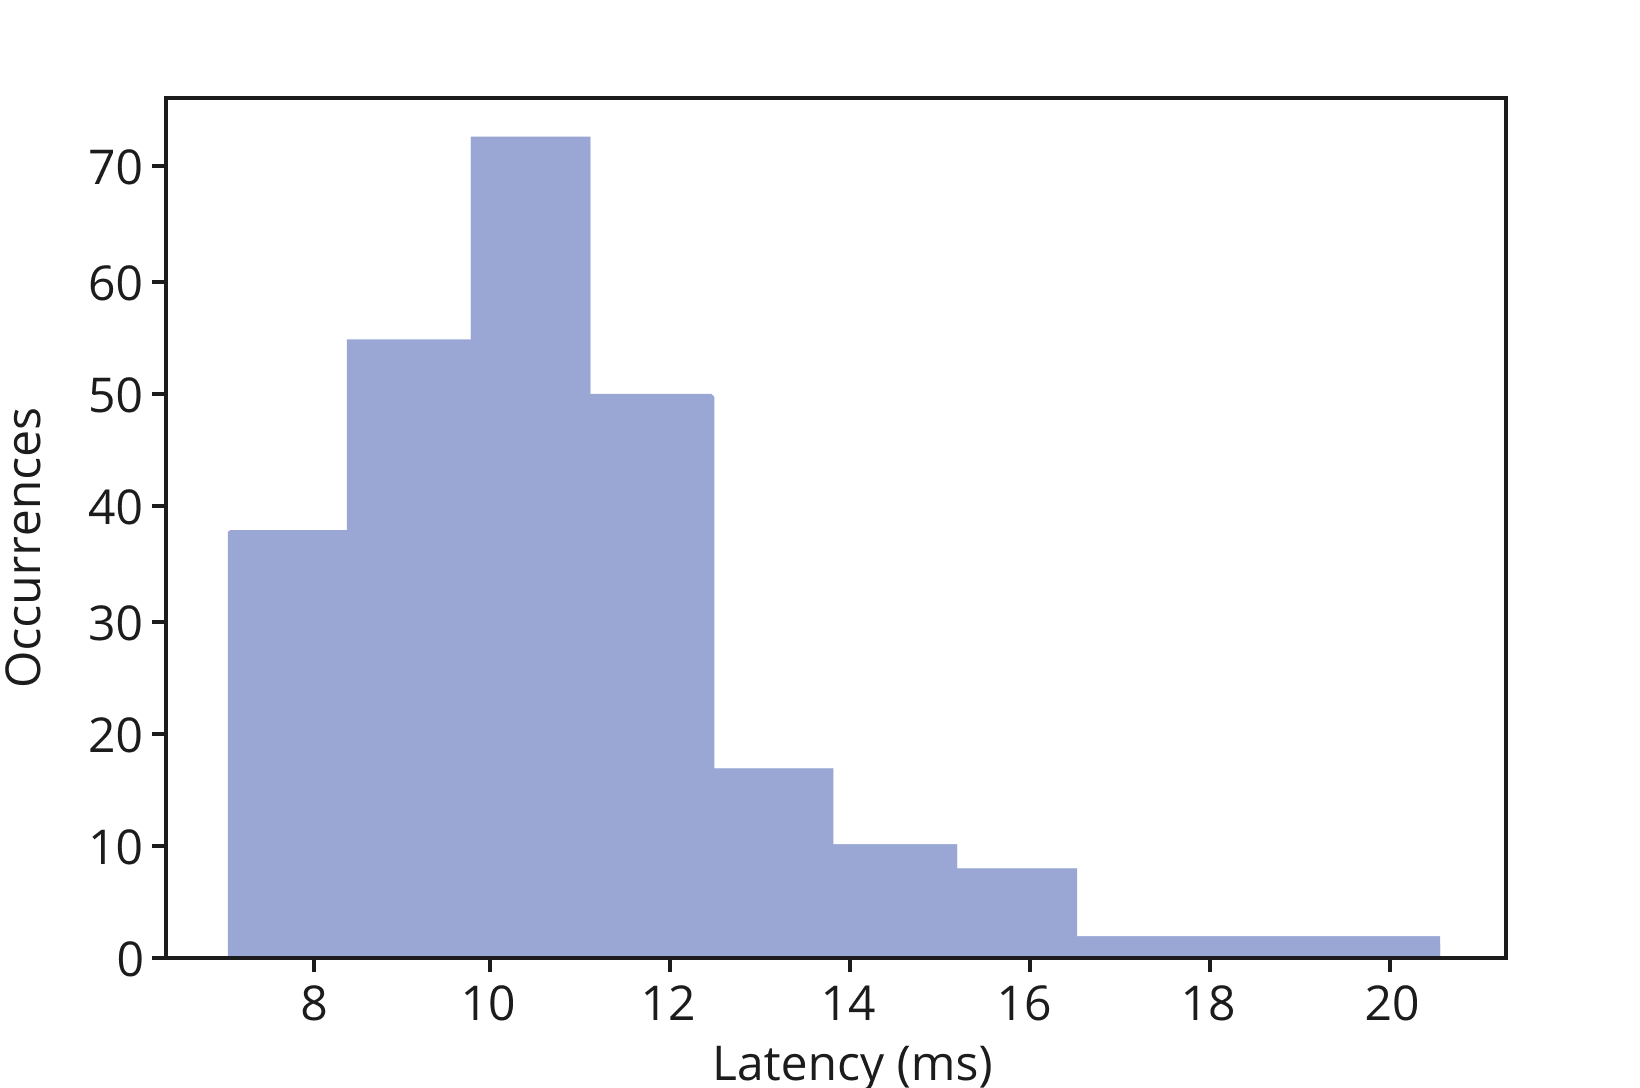
\includegraphics[width=0.7\textwidth]{Chapters/Figures/technical/Latency/figure3.png}
    \caption{Latency results for one device (1 metre).}
    \label{fig:latency_fig3}
\end{figure}

\subsection*{Multiple Devices}

% \subsection*{Configuration}
For the following, we report our results when using 4 devices simultaneously. To test multiple devices, we pair each R-IoT to the same router and separate the incoming data according to the ID number of the device. All devices are sending data to the same port number. Other conditions are kept the same as the previous test.

% \subsection*{Data Analysis}

\subsubsection*{Absolute Latency}
The minimum, maximum and mean latency measures for the individual devices are shown in Table \ref{table:latency_tab3} and \ref{table:latency_tab4}. We can see the maximum and mean latency has increased in all instances when more devices are added to the network. The results are fairly consistent between each device aside from device ID 2, which doesn’t reach as high of a maximum. From all 992 triggers, the latency durations ranged from 6.55 to 17.31 milliseconds, and the mean average was calculated as 10.03 milliseconds. We present these results as a histogram in Figure \ref{fig:latency_fig4} and Figure \ref{fig:latency_fig5}. When we repeat the test at 5 metres, we identified a small increase in the average latency and a higher maximum amongst all the devices.

% Table 3
% \begin{table}[!h]
%     \centering
%     \begin{tabular}{*{4}{l}}\hline
%     % \rowcolor[HTML]{34CDF9}
%     \textbf{Device ID} & \textbf{\begin{tabular}[c]{@{}l@{}}Maximum\\ Latency (ms)\end{tabular}} & \textbf{\begin{tabular}[c]{@{}l@{}}Minimum\\ Latency (ms)\end{tabular}} & \textbf{\begin{tabular}[c]{@{}l@{}}Mean\\ Latency (ms)\end{tabular}} \\
%     \\[-1em]
%     \hline
%     \\[-1em]
%     0                  & 11.019                        & 6.605                & 8.859\\
%     \\[-1em]
%     \hline
%     \end{tabular}
% \caption{Latency results for one device (1 metre).}
% \label{table:latency_tab3}
% \end{table}

\begin{table}[htbp]
    \begin{subtable}[c]{\textwidth}
        \centering
            \begin{tabular}{*{4}{l}}\hline
            % \rowcolor[HTML]{34CDF9}
            \textbf{Device ID} & \textbf{\begin{tabular}[c]{@{}l@{}}Maximum\\ Latency (ms)\end{tabular}} & \textbf{\begin{tabular}[c]{@{}l@{}}Minimum\\ Latency (ms)\end{tabular}} & \textbf{\begin{tabular}[c]{@{}l@{}}Mean\\ Latency (ms)\end{tabular}} \\
            \\[-1em]
            \hline
            \\[-1em]
            0                  & 16.243                                                                  & 6.705                                                                   & 10.011                                                               \\
            \\[-1em]
            1                  & 17.201                                                                  & 6.657                                                                   & 10.007                                                               \\
            \\[-1em]
            2                  & 14.877                                                                  & 6.550                                                                   & 9.998                                                                \\
            \\[-1em]
            3                  & 17.305                                                                  & 6.868                                                                   & 10.130  \\
            \\[-1em]
            \hline
            \end{tabular}
        \caption{Latency at 1 metre.}
        \label{table:latency_tab3}
    \end{subtable}
    \hfill
    % \hspace{2em}
    \caption{Latency measurements for four devices.}
    \label{table:latency_four_devices}
\end{table}

% Figure 4
\begin{figure}[htbp]
  \centering
    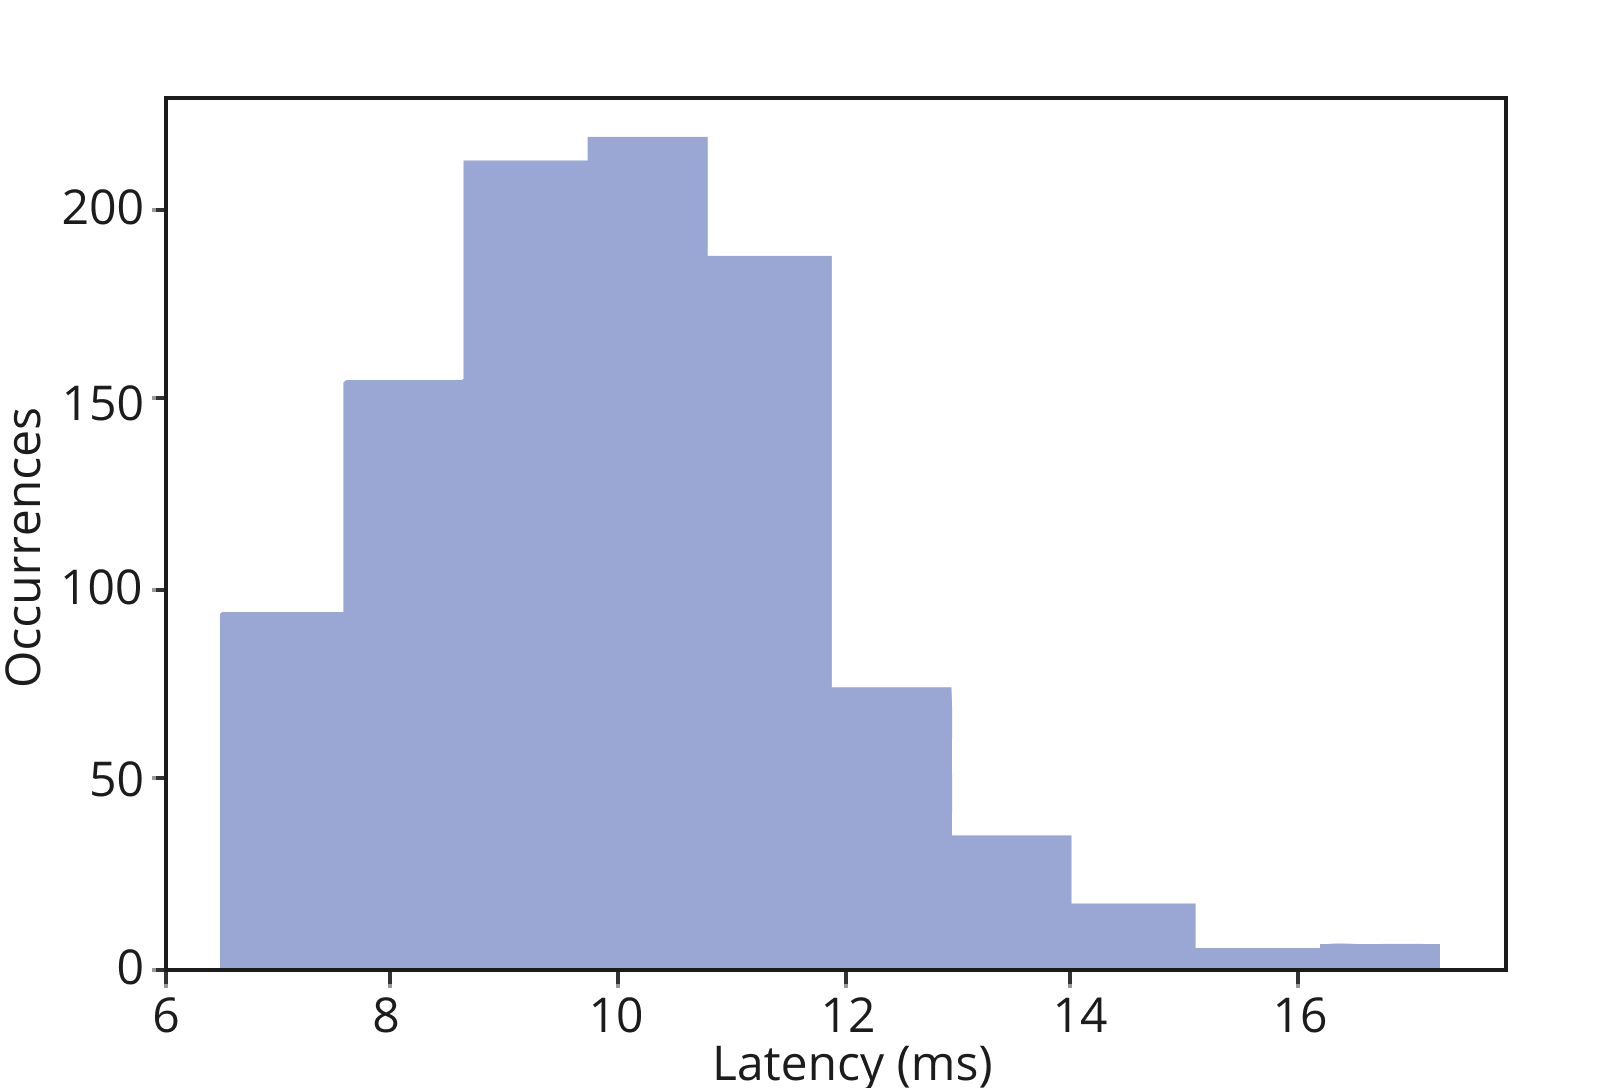
\includegraphics[width=0.7\textwidth]{Chapters/Figures/technical/Latency/figure4.png}
    \caption{Latency results for one device (1 metre).}
    \label{fig:latency_fig4}
\end{figure}

% Table 4
\begin{table}[htbp]
    \begin{subtable}[c]{\textwidth}
        \centering
            \begin{tabular}{*{4}{l}}\hline
            % \rowcolor[HTML]{34CDF9}
            \textbf{Device ID} & \textbf{\begin{tabular}[c]{@{}l@{}}Maximum\\ Latency (ms)\end{tabular}} & \textbf{\begin{tabular}[c]{@{}l@{}}Minimum\\ Latency (ms)\end{tabular}} & \textbf{\begin{tabular}[c]{@{}l@{}}Mean\\ Latency (ms)\end{tabular}} \\
            \\[-1em]
            \hline
            \\[-1em]
            0                  & 27.992                                                                  & 6.720                                                                   & 11.023                                                               \\                                                               \\
            \\[-1em]
            1                  & 27.559                                                                  & 7.248                                                                   & 11.916                                                               \\
            \\[-1em]
            2                  & 27.990                                                                  & 6.857                                                                   & 11.263                                                               \\
            \\[-1em]
            3                  & 26.346                                                                  & 6.837                                                                   & 10.830 \\
            \\[-1em]
            \hline
            \end{tabular}
        \caption{Latency at 5 metres.}
        \label{table:latency_tab4}
    \end{subtable}
    \hfill
    % \hspace{2em}
    \caption{Latency measurements for four devices.}
    \label{table:latency_four_devices_2}
\end{table}

% \begin{table}[h]
%     \begin{subtable}[c]{\textwidth}
%         \centering
%             \begin{tabular}{*{4}{l}}\hline
%             % \rowcolor[HTML]{34CDF9}
%             \textbf{Device ID} & \textbf{\begin{tabular}[c]{@{}l@{}}Maximum\\ Latency (ms)\end{tabular}} & \textbf{\begin{tabular}[c]{@{}l@{}}Minimum\\ Latency (ms)\end{tabular}} & \textbf{\begin{tabular}[c]{@{}l@{}}Mean\\ Latency (ms)\end{tabular}} \\
%             \\[-1em]
%             \hline
%             \\[-1em]
%             0                  & 11.019                        & 6.605                & 8.859\\
%             \\[-1em]
%             \hline
%             \end{tabular}
%         \caption{Latency at 5 metres.}
%         \label{table:latency_tab4}
%     \end{subtable}
%     \hfill
%     % \hspace{2em}
%     \caption{Latency measurements for four devices.}
%     \label{table:latency_four_devices}
% \end{table}

% Figure 5 Histogram of absolute latencies (5 metres)
\begin{figure}[htbp]
  \centering
    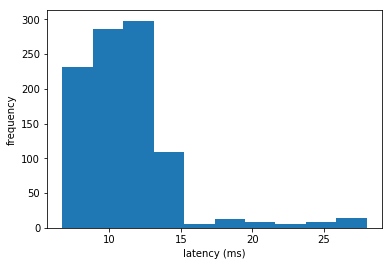
\includegraphics[width=0.7\textwidth]{Chapters/Figures/technical/Latency/figure5.png}
    \caption{Latency results for one device (1 metre).}
    \label{fig:latency_fig5}
\end{figure}

\subsubsection*{Relative Latency}

As well as the response time between each individual device and the host computer, we are also interested in the difference in latency of the received message between all the devices in the network. This is important to enable data synchronisation between sources. For each trigger, we calculate the difference between the first and the last response out of the 4 devices. From our first acquisition, the mean average latency difference was calculated as 3.22 milliseconds with a maximum 8.96. In Figure~\ref{fig:latency_fig6} and \ref{fig:latency_fig7} the data is plotted as a histogram to assess the likelihood of these latency differences occurring. When we increase the distance, we find the maximum relative latency goes up to 20.148 milliseconds, and we calculate an increased average of 5.925 milliseconds.

% Figure 6
\begin{figure}[htbp]
  \centering
    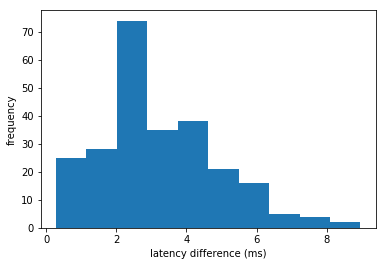
\includegraphics[width=0.7\textwidth]{Chapters/Figures/technical/Latency/figure6.png}
    \caption{Latency results for one device (1 metre).}
    \label{fig:latency_fig6}
\end{figure}

% Figure 7
\begin{figure}[htbp]
  \centering
    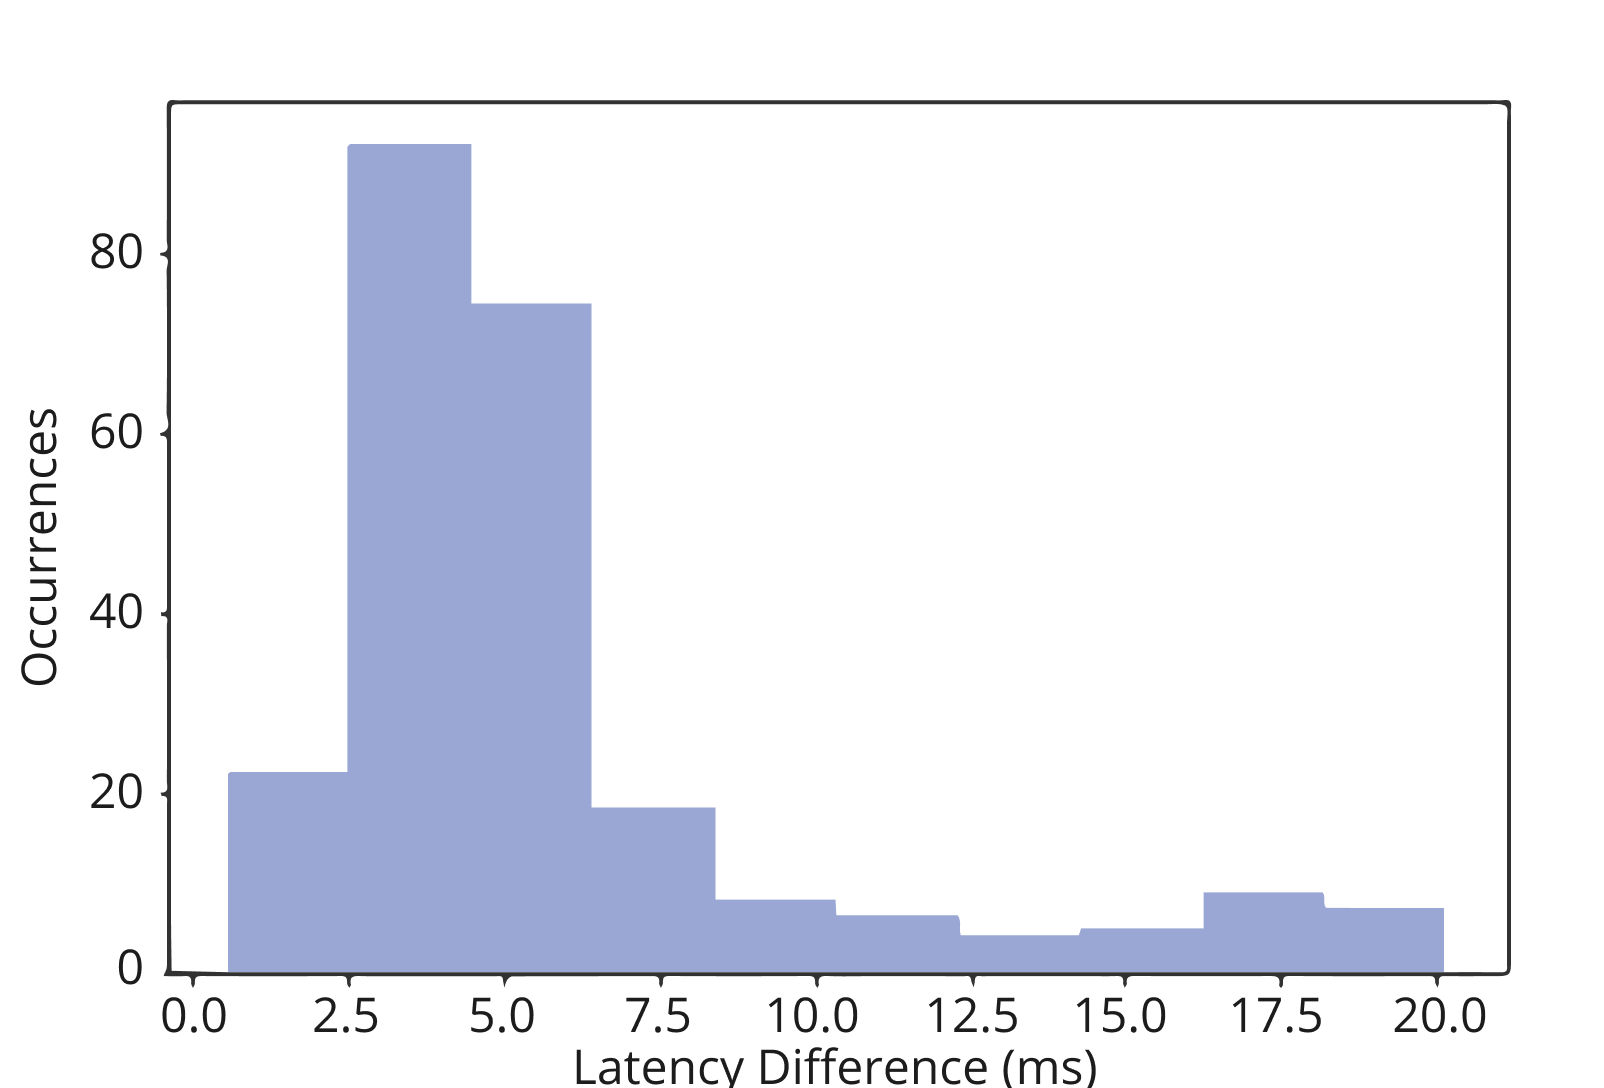
\includegraphics[width=0.7\textwidth]{Chapters/Figures/technical/Latency/figure7.png}
    \caption{Latency results for one device (1 metre).}
    \label{fig:latency_fig7}
\end{figure}

\subsection{Summary}

\subsection*{Limitations}
\label{subsec:latency_limitations}
There are a couple of factors regarding wireless configuration that are worth noting. First is that all the devices were sending data to the same port number (8888). We did this for convenience and ease of programming. However, we acknowledge that separating ports for each device may have an effect of performance, as advised in the official documentation \cite{noauthor_bitalino_nodate}. Secondly, we set a WPA-2 password on the network which uses more bandwidth. Another factor that is briefly addressed in the document is the added latency between the host computer and the Teensy 3.2, connected by USB. As the communication was dependent on single byte messages, we assume that this is negligible to the final results\footnote{Serial Latency: \url{http://neophob.com/2011/04/serial-latency-teensy-vs-arduino/}}.

\subsection*{Latency Assessment}

From the results, we conclude the following factors to have an impact on the latency between the R-IoT and the host computer. Having more devices in the network will increase the average latency and maximum latency. Additionally, increasing the distance between the R-IoT(s) and the Wi-Fi router will also increase the average latency. When we tested four devices at 5 metres, we observed a few instances of the latency being much higher than the average, compared to when we tested at a short distance. We also found that the distance would affect the difference in latency between devices, which would have an impact on data synchronization.
